\chapter{Results and Discussion}
\label{chapter:results_and_discussion}

\section{Usability}
\label{section:usability}
%  more info on usability score: https://measuringu.com/sus/
% A SUS score above 68 would be considered above average, and anything below 68 is below average.
% # A SUS score of 74 has higher perceived usability than 70\% of all products tested. It can be interpreted as a grade of a B-.

The post-study usability questionnaire resulted in an average SUS score of 81.1 across all five participants (see \autoref{table:sus}). According to \textcite{sauroSUS}, one would need to score above 80.3 to be in the top 10\% of the 500 studies using the SUS. 80.3 is also the point where users are more likely to be recommending the product to a friend \autocite{sauroSUS}, making us believe that AmbientTeams was easy and intuitive to use.

TODO: Likert-Scale chart and remove Q1-Q10 from SUS score table

\begin{table}[h]
    \centering
    \begin{tabular}{|l c c c c c c c c c c l|}
        \hline
        Participant & Q1 & Q2 & Q3 & Q4 & Q5 & Q6 & Q7 & Q8 & Q9 & Q10 & SUS score \\
        \hline
        P038        & 3  & 1  & 4  & 1  & 3  & 1  & 5  & 1  & 5  & 3   & 82.5      \\
        % \hline
        P163        & 4  & 1  & 4  & 4  & 5  & 1  & 5  & 1  & 5  & 4   & 80.0      \\
        % \hline
        P586        & 2  & 2  & 5  & 1  & 2  & 3  & 5  & 3  & 4  & 1   & 70.0      \\
        % \hline
        P751        & 5  & 2  & 4  & 1  & 4  & 2  & 5  & 2  & 4  & 2   & 82.5      \\
        % \hline
        P904        & 4  & 1  & 4  & 1  & 4  & 1  & 5  & 1  & 4  & 1   & 90.5      \\
        % \hline
        Average     &    &    &    &    &    &    &    &    &    &     & 81.1      \\
        \hline
    \end{tabular}
    \caption{Usability questionnaire results and resulting SUS score}
    \label{table:sus}
\end{table}

\section{Tool Usage and Workflows (RQ4)}
\label{section:tool_usage_and_workflows}

A detailed timeline view of the participants and their selected availability state ("Avaiable", "Focused", or "Happy to interact") are visualized in \autoref{fig:non_offline}. Those three states combined are looked at as the time when the application was adequately running (potentially in the background). This is because the user is automatically set to an offline state if the connection to the server is lost. Upon successful connection to the server, the users' availability state is also automatically set to "Available". It is worth mentioning that this metric could be slightly erroneous if participants manually set their availability status to "Offline". This would, however, only underestimate the time spent online in \autoref{fig:non_offline}, making our results as conservative as possible. All in all, the average time spent in a non-offline state, and thus AmbientTeams was running (potentially only in the background), was 7.13 hours per day (std. 3.57), with a minimum of 0 and a maximum of 12.7 hours. Except for the inactivity on the weekend, only some participants did not use AmbientTeams some days. To be precise, only 5 out of a total of 30 workdays showed no or very little running time. The fact that P038 could not participate in the initial meeting with the rest of the group explains the lack of usage on the first day of the study. In general, because the kick-off meeting took place in the early afternoon, the relatively short running time on the first day was to be expected. The remaining days with very little only time most likely indicate non-working days for those participants because had they worked on those days, AmbientTeams would have automatically started as soon as they had started up their computer.

\begin{figure}[h]
    \centering
    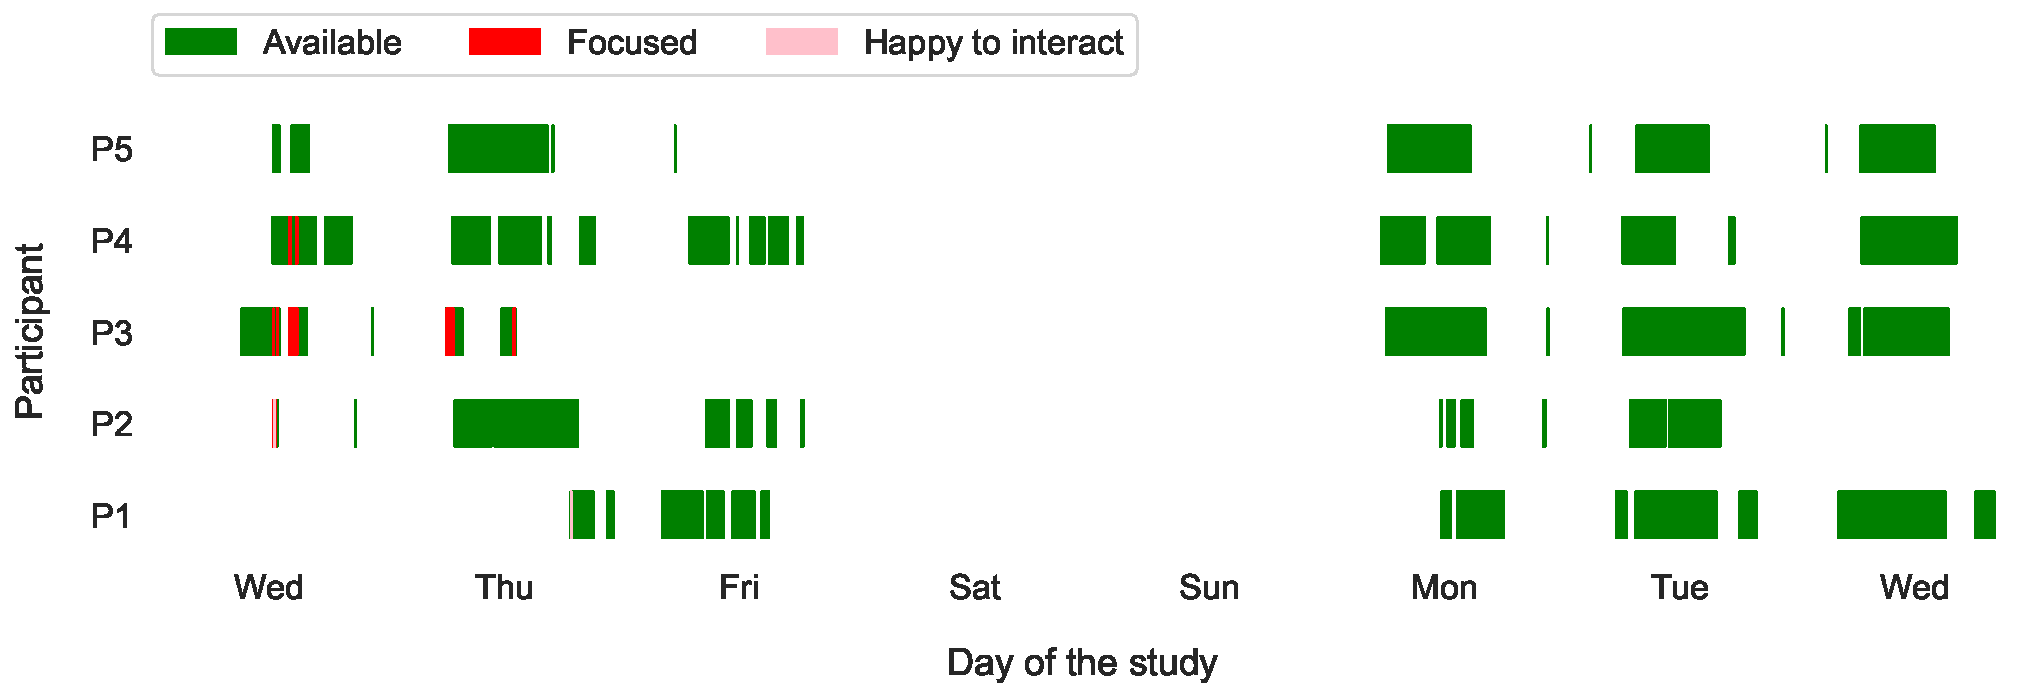
\includegraphics[width=\linewidth]{plots/non_offline.pdf}
    \caption{Time spent in the different availability states}
    \label{fig:non_offline}
\end{figure}

The results show that the participants did not often change their availability states and thus mainly relied on the automatic availability status setting of AmbientTeams. The "Focused" state was selected a couple of times in the first two days of the study, yet this behavior did not continue throughout the study.


\subsection{Little Active Use}
As with the changes in availability status, many interactions recorded with AmbientTeams were rather unspectacular. \autoref{fig:opened_vs_focused} illustrates that both the ambient window and the team overview window were almost exclusively opened when those windows were in focus. In other words, both of those windows were opened, interaction took place, and then they were closed or minimized again, making them disappear from the user's monitor. This is the result we expected to happen in the case of the team overview. In contrast to our beliefs, however, the ambient window was used very similarly. As a result, the ambient window only very rarely was kept open as a glanceable, always-on-top team view when working on other tasks.

\begin{figure}[h]
    \centering
    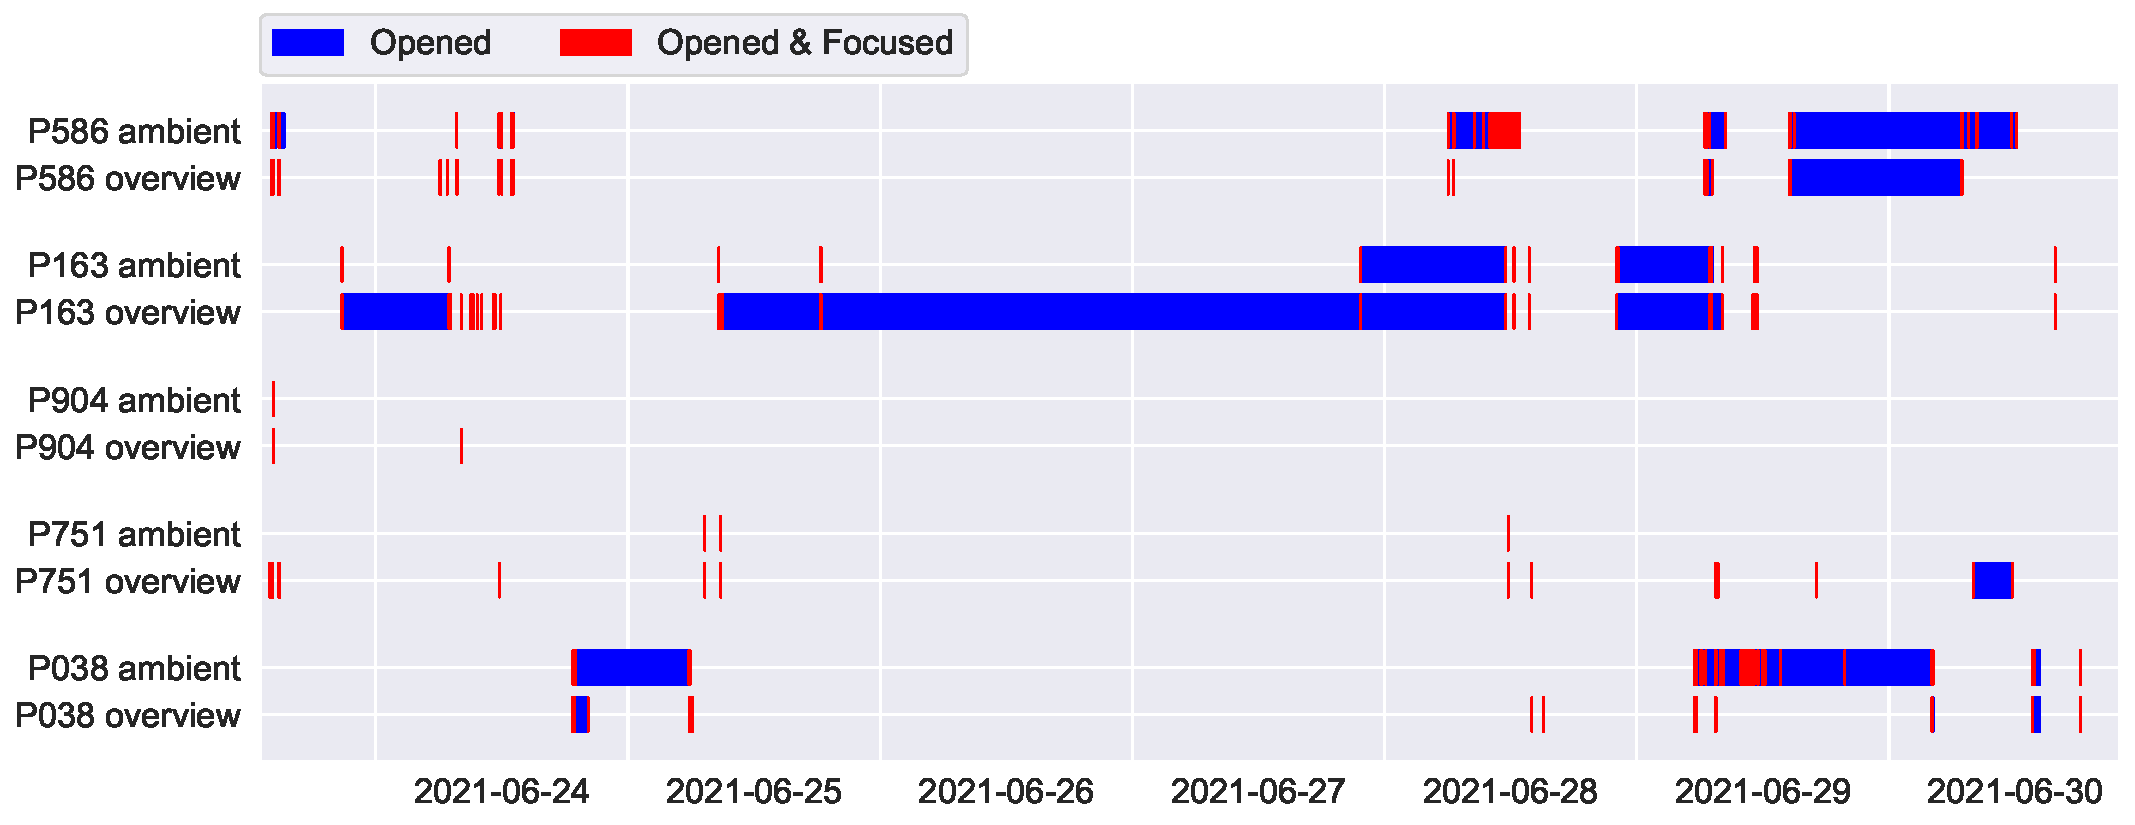
\includegraphics[width=\linewidth]{plots/open_vs_focus.pdf}
    \caption{Time AmbientTeams was opened vs. opened and focused}
    \label{fig:opened_vs_focused}
\end{figure}

The interviews gave us some more insights into possible answers for why the ambient window was not kept open while working on other tasks:

\begin{displayquote}
    I tried it in the corner of the monitor, then it did not work, but in the corner of the window did not really work because there you have to click to close other windows. Then I put it somewhere in the middle, but then I needed to put some buttons there, so sometimes I got annoyed and then closed it. -P038
\end{displayquote}

We hypothesize that this particular user most likely was using a single monitor setup and had a hard time finding a suitable position for the ambient window. The participant further presented a potential solution to the problem:

P586 mentioned that the ambient window was too small and thus too difficult to properly move around, indicating that this participant might have missed this part of the demonstration during the kick-off meeting. In addition to the annoyance of the ambient window experienced by P038 and P586, P163 mentioned that manually closing an application that automatically starts up is something that happens almost automatically to them. The hassle and difficulties of positioning the ambient window are a rather crucial issue that potentially requires further development; the case described by P163 could be solved by not allowing to close the ambient window during a future study.

To make the ambient window fit better into their workflow, P038 suggested that it should ideally not stay on top of other windows and instead just come to the foreground again once a team member has shared something new.

Despite the criticism around the ambient window, it was still used by all the participants except for P904 and seen as one of the best aspects of AmbientTeams by P751:

\begin{displayquote}
    I liked that the ambient window feels very dynamic and refreshing compared to other tools. -P751
\end{displayquote}

Despite this positive statement, this participant used the team overview window more, which is surprising because all the participants were only part of one team during the study, eliminating the potential advantage of the team overview window, in our opinion.

Considering the relatively short time AmbientTeams was actively used, it is not surprising that many of its features were not used. More concretely, the features aimed at spontaneous interactions such as the breakroom and the random pairing for a video call were not used at all. While there have been two attempts of creating a breakroom, one on the second day of the study and one on the second to last day, none of them were sucessfully created because no other team member joined. P586 gave a possible explanation for why the spontaneous video chat features were not used during the interview.

\begin{displayquote}
    But also maybe I have to mention that two or three weeks ago we started with virtual break rooms on Friday afternoons to try to keep up with people from work, especially for new people, because we don't really get the chance to get to know each other in home office. -P586
\end{displayquote}

Consequently, it is possible that it is sufficient for the participating teams to meet once a week in their own virtual break room. Regardless of the use of the break room integrated into AmbientTeams, this indicates that the concept of such a break room is generally perceived as important. Similar to the breakroom, the directed video calls and the nudging functionality were only used during the initial kick-off meeting for testing purposes. While this shows that it was clear to the team how to use those features, they don't seem to have felt the need for those.

Things look a bit different when analyzing the direct messages that were sent through AmbientTeams. In total, there were six direct messages sent through AmbientTeams, coming from three different participants. One of those direct messages was a response to a missed call, and the other five were of either of type greeting or along the lines of "what are you doing?". P032 gives an indication to why the team did not use the above-described functionalities:

\begin{displayquote}
    Because now it's a bit, you know I can write to somebody in Microsoft Teams or AmbientTeams, and I would normally pick MS Teams because we use it, and you also have a message history which you don't have in AmbientTeams.
    -P032
\end{displayquote}

Essentially, P032 explains that AmbientTeams has to differentiate itself from MS Teams, and it is doing so with the \textit{Twitter approach} of broadcasting moods and messages, but not so much with other communication functionalities.

When it comes to sharing moods and status messages, eight status messages were shared, three of which were in reaction to Switzerland's soccer game during that time. Generally speaking, none of the status messages contained any work-related information.

\begin{figure}[h]
    \centering
    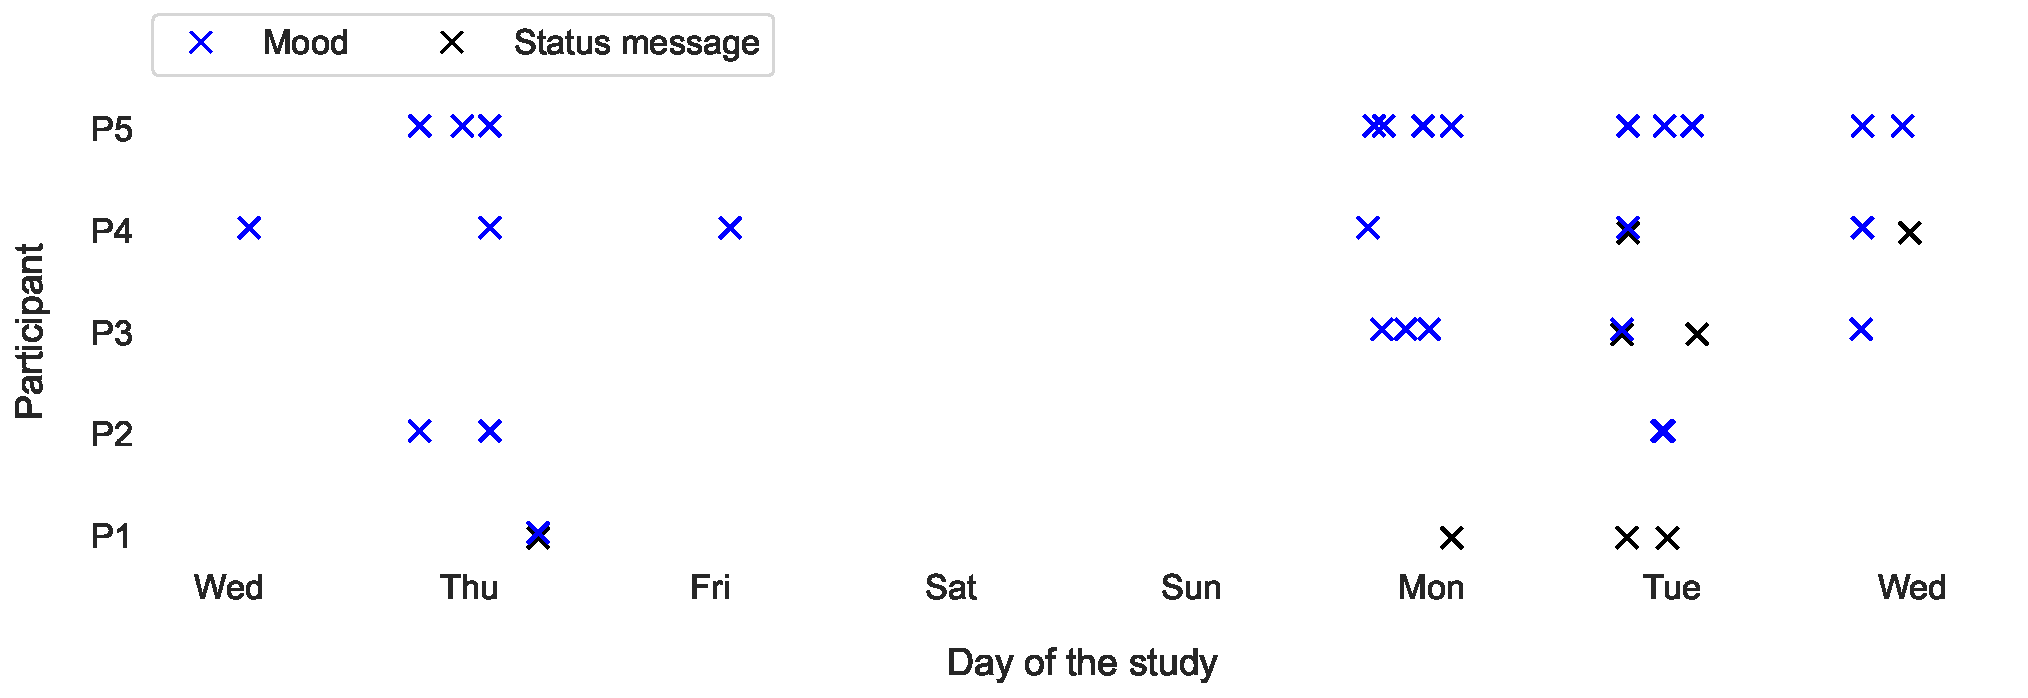
\includegraphics[width=\linewidth]{plots/moods_status_messages.pdf}
    \caption{Moods and status messages shared}
    \label{fig:moods_status_messages}
\end{figure}

To conclude, despite the high SUS score, the data shows that AmbientTeams was used in the sense that it ran in the background, but various functionalities were only used to a limited extent, or not at all. The more commonly used micro-blogging functionality, on which also the study put more emphasis, is discussed in the following section.


\section{Micro-Blogging: Sharing Moods and Status Messages}
\label{section:micro_blogging}

\subsection{A Need for Status and Mood Sharing (RQ1)}

\textbf{Lack of Awareness} \\
We asked the participants why and how they used AmbientTeams during the study. Two reasons for checking AmbientTeams could have been identified, highlighting the interests in states of other team members, namely moods, status messages, and availability.

% \begin{displayquote}
%     I mainly used it to check who is online and still around and sometimes to ask how they feel. \\
%     -P038
% \end{displayquote}

\begin{displayquote}
    Also, sometimes for just checking who is online and who is grayed out. \\
    -P586
\end{displayquote}

\begin{displayquote}
    I think it was very interesting to see moods and states of team members with whom I might not be currently working together too closely. \\
    -P751
\end{displayquote}

\begin{displayquote}
    I think it's a good idea, especially now if you work either hybrid or completely remote, I think then it is quite difficult to see the mood of your team colleagues, because now in most video conferences you make a happy face into the camera, so it is also difficult to see your mood how your mood really is right now. \\
    -P163
\end{displayquote}

\begin{displayquote}
    Sometimes I then [at a previous company] got the feedback that they already finished with work or that that they have no more tasks left. With something like AmbientTeams they could set like a bored state and I would have been able to give them a new task. \\
    -P163
\end{displayquote}

\begin{displayquote}
    I very much like the idea of sharing moods with the team. As we are becoming more aware on such a sensitive topic as mental health, this feature allows to discover more about your colleagues, and it sheds light to a part that we tend to keep only for ourselves. \\
    -P751
\end{displayquote}

This finding confirms a lack of awareness when working remotely and shows a general interest in the moods and feelings of co-workers. It seems to be a known fact amongst the participants that talking about feelings is important. However, P586 also expressed some concerns about a mood sharing approach:

\begin{displayquote}
    I mean of course it is very important that you talk about these kinds of things [feelings], but you don't want to share it with the whole team. \\
    -P586
\end{displayquote}

TODO: Pre-study questionnaire results regarding lack of awareness

\textbf{Lack of social contact / task-focus} \\

\begin{displayquote}
    I think during corona, you don't really have that breakroom time, so if you call somebody, it's mostly about business and not about private stuff. So, I think it's very difficult to get into a deeper connection with people you don't see that often. \\
    -P586
\end{displayquote}

\subsubsection{Motivation for Sharing}
Maybe don't put in separate subsubsection, have to see


\subsection{What Is Shared and Why? (RQ2)}





\section{Effects (RQ3)}
\label{section:effects}

\section{Workplace Isolation}
\label{section:workplace_isolation}

\section{Broader Tool Feedback and Future Directions}
\label{section:feedback_future_directions}

\subsection{Better Integration with Established Tools}
To increase the use and usage of AmbientTeams, participants Pxxx, Pxxx, and Pxxx all mentioned that a single tool would increase the likelihood and time they would use our mood-based micro-blogging approach.

\begin{displayquote}
    I think it would be good if AT could be integrated into Teams because if you have one tool, then you would use it more often. -P163
\end{displayquote}

\subsection{Improved Tool Feedback}

\subsection{Self-Reflection}

\subsection{Task-Sharing}


Generally, x/y said that they would continue using it. X would continue using it if xyz was changed.